% Options for packages loaded elsewhere
\PassOptionsToPackage{unicode}{hyperref}
\PassOptionsToPackage{hyphens}{url}
\PassOptionsToPackage{dvipsnames,svgnames,x11names}{xcolor}
%
\documentclass[
  letterpaper,
  DIV=11,
  numbers=noendperiod]{scrartcl}

\usepackage{amsmath,amssymb}
\usepackage{lmodern}
\usepackage{iftex}
\ifPDFTeX
  \usepackage[T1]{fontenc}
  \usepackage[utf8]{inputenc}
  \usepackage{textcomp} % provide euro and other symbols
\else % if luatex or xetex
  \usepackage{unicode-math}
  \defaultfontfeatures{Scale=MatchLowercase}
  \defaultfontfeatures[\rmfamily]{Ligatures=TeX,Scale=1}
\fi
% Use upquote if available, for straight quotes in verbatim environments
\IfFileExists{upquote.sty}{\usepackage{upquote}}{}
\IfFileExists{microtype.sty}{% use microtype if available
  \usepackage[]{microtype}
  \UseMicrotypeSet[protrusion]{basicmath} % disable protrusion for tt fonts
}{}
\makeatletter
\@ifundefined{KOMAClassName}{% if non-KOMA class
  \IfFileExists{parskip.sty}{%
    \usepackage{parskip}
  }{% else
    \setlength{\parindent}{0pt}
    \setlength{\parskip}{6pt plus 2pt minus 1pt}}
}{% if KOMA class
  \KOMAoptions{parskip=half}}
\makeatother
\usepackage{xcolor}
\usepackage[normalem]{ulem}
\setlength{\emergencystretch}{3em} % prevent overfull lines
\setcounter{secnumdepth}{-\maxdimen} % remove section numbering
% Make \paragraph and \subparagraph free-standing
\ifx\paragraph\undefined\else
  \let\oldparagraph\paragraph
  \renewcommand{\paragraph}[1]{\oldparagraph{#1}\mbox{}}
\fi
\ifx\subparagraph\undefined\else
  \let\oldsubparagraph\subparagraph
  \renewcommand{\subparagraph}[1]{\oldsubparagraph{#1}\mbox{}}
\fi

\usepackage{color}
\usepackage{fancyvrb}
\newcommand{\VerbBar}{|}
\newcommand{\VERB}{\Verb[commandchars=\\\{\}]}
\DefineVerbatimEnvironment{Highlighting}{Verbatim}{commandchars=\\\{\}}
% Add ',fontsize=\small' for more characters per line
\usepackage{framed}
\definecolor{shadecolor}{RGB}{241,243,245}
\newenvironment{Shaded}{\begin{snugshade}}{\end{snugshade}}
\newcommand{\AlertTok}[1]{\textcolor[rgb]{0.68,0.00,0.00}{#1}}
\newcommand{\AnnotationTok}[1]{\textcolor[rgb]{0.37,0.37,0.37}{#1}}
\newcommand{\AttributeTok}[1]{\textcolor[rgb]{0.40,0.45,0.13}{#1}}
\newcommand{\BaseNTok}[1]{\textcolor[rgb]{0.68,0.00,0.00}{#1}}
\newcommand{\BuiltInTok}[1]{\textcolor[rgb]{0.00,0.23,0.31}{#1}}
\newcommand{\CharTok}[1]{\textcolor[rgb]{0.13,0.47,0.30}{#1}}
\newcommand{\CommentTok}[1]{\textcolor[rgb]{0.37,0.37,0.37}{#1}}
\newcommand{\CommentVarTok}[1]{\textcolor[rgb]{0.37,0.37,0.37}{\textit{#1}}}
\newcommand{\ConstantTok}[1]{\textcolor[rgb]{0.56,0.35,0.01}{#1}}
\newcommand{\ControlFlowTok}[1]{\textcolor[rgb]{0.00,0.23,0.31}{#1}}
\newcommand{\DataTypeTok}[1]{\textcolor[rgb]{0.68,0.00,0.00}{#1}}
\newcommand{\DecValTok}[1]{\textcolor[rgb]{0.68,0.00,0.00}{#1}}
\newcommand{\DocumentationTok}[1]{\textcolor[rgb]{0.37,0.37,0.37}{\textit{#1}}}
\newcommand{\ErrorTok}[1]{\textcolor[rgb]{0.68,0.00,0.00}{#1}}
\newcommand{\ExtensionTok}[1]{\textcolor[rgb]{0.00,0.23,0.31}{#1}}
\newcommand{\FloatTok}[1]{\textcolor[rgb]{0.68,0.00,0.00}{#1}}
\newcommand{\FunctionTok}[1]{\textcolor[rgb]{0.28,0.35,0.67}{#1}}
\newcommand{\ImportTok}[1]{\textcolor[rgb]{0.00,0.46,0.62}{#1}}
\newcommand{\InformationTok}[1]{\textcolor[rgb]{0.37,0.37,0.37}{#1}}
\newcommand{\KeywordTok}[1]{\textcolor[rgb]{0.00,0.23,0.31}{#1}}
\newcommand{\NormalTok}[1]{\textcolor[rgb]{0.00,0.23,0.31}{#1}}
\newcommand{\OperatorTok}[1]{\textcolor[rgb]{0.37,0.37,0.37}{#1}}
\newcommand{\OtherTok}[1]{\textcolor[rgb]{0.00,0.23,0.31}{#1}}
\newcommand{\PreprocessorTok}[1]{\textcolor[rgb]{0.68,0.00,0.00}{#1}}
\newcommand{\RegionMarkerTok}[1]{\textcolor[rgb]{0.00,0.23,0.31}{#1}}
\newcommand{\SpecialCharTok}[1]{\textcolor[rgb]{0.37,0.37,0.37}{#1}}
\newcommand{\SpecialStringTok}[1]{\textcolor[rgb]{0.13,0.47,0.30}{#1}}
\newcommand{\StringTok}[1]{\textcolor[rgb]{0.13,0.47,0.30}{#1}}
\newcommand{\VariableTok}[1]{\textcolor[rgb]{0.07,0.07,0.07}{#1}}
\newcommand{\VerbatimStringTok}[1]{\textcolor[rgb]{0.13,0.47,0.30}{#1}}
\newcommand{\WarningTok}[1]{\textcolor[rgb]{0.37,0.37,0.37}{\textit{#1}}}

\providecommand{\tightlist}{%
  \setlength{\itemsep}{0pt}\setlength{\parskip}{0pt}}\usepackage{longtable,booktabs,array}
\usepackage{calc} % for calculating minipage widths
% Correct order of tables after \paragraph or \subparagraph
\usepackage{etoolbox}
\makeatletter
\patchcmd\longtable{\par}{\if@noskipsec\mbox{}\fi\par}{}{}
\makeatother
% Allow footnotes in longtable head/foot
\IfFileExists{footnotehyper.sty}{\usepackage{footnotehyper}}{\usepackage{footnote}}
\makesavenoteenv{longtable}
\usepackage{graphicx}
\makeatletter
\def\maxwidth{\ifdim\Gin@nat@width>\linewidth\linewidth\else\Gin@nat@width\fi}
\def\maxheight{\ifdim\Gin@nat@height>\textheight\textheight\else\Gin@nat@height\fi}
\makeatother
% Scale images if necessary, so that they will not overflow the page
% margins by default, and it is still possible to overwrite the defaults
% using explicit options in \includegraphics[width, height, ...]{}
\setkeys{Gin}{width=\maxwidth,height=\maxheight,keepaspectratio}
% Set default figure placement to htbp
\makeatletter
\def\fps@figure{htbp}
\makeatother

\KOMAoption{captions}{tableheading}
\makeatletter
\@ifpackageloaded{tcolorbox}{}{\usepackage[many]{tcolorbox}}
\@ifpackageloaded{fontawesome5}{}{\usepackage{fontawesome5}}
\definecolor{quarto-callout-color}{HTML}{909090}
\definecolor{quarto-callout-note-color}{HTML}{0758E5}
\definecolor{quarto-callout-important-color}{HTML}{CC1914}
\definecolor{quarto-callout-warning-color}{HTML}{EB9113}
\definecolor{quarto-callout-tip-color}{HTML}{00A047}
\definecolor{quarto-callout-caution-color}{HTML}{FC5300}
\definecolor{quarto-callout-color-frame}{HTML}{acacac}
\definecolor{quarto-callout-note-color-frame}{HTML}{4582ec}
\definecolor{quarto-callout-important-color-frame}{HTML}{d9534f}
\definecolor{quarto-callout-warning-color-frame}{HTML}{f0ad4e}
\definecolor{quarto-callout-tip-color-frame}{HTML}{02b875}
\definecolor{quarto-callout-caution-color-frame}{HTML}{fd7e14}
\makeatother
\makeatletter
\makeatother
\makeatletter
\makeatother
\makeatletter
\@ifpackageloaded{caption}{}{\usepackage{caption}}
\AtBeginDocument{%
\ifdefined\contentsname
  \renewcommand*\contentsname{Table of contents}
\else
  \newcommand\contentsname{Table of contents}
\fi
\ifdefined\listfigurename
  \renewcommand*\listfigurename{List of Figures}
\else
  \newcommand\listfigurename{List of Figures}
\fi
\ifdefined\listtablename
  \renewcommand*\listtablename{List of Tables}
\else
  \newcommand\listtablename{List of Tables}
\fi
\ifdefined\figurename
  \renewcommand*\figurename{Figure}
\else
  \newcommand\figurename{Figure}
\fi
\ifdefined\tablename
  \renewcommand*\tablename{Table}
\else
  \newcommand\tablename{Table}
\fi
}
\@ifpackageloaded{float}{}{\usepackage{float}}
\floatstyle{ruled}
\@ifundefined{c@chapter}{\newfloat{codelisting}{h}{lop}}{\newfloat{codelisting}{h}{lop}[chapter]}
\floatname{codelisting}{Listing}
\newcommand*\listoflistings{\listof{codelisting}{List of Listings}}
\makeatother
\makeatletter
\@ifpackageloaded{caption}{}{\usepackage{caption}}
\@ifpackageloaded{subcaption}{}{\usepackage{subcaption}}
\makeatother
\makeatletter
\@ifpackageloaded{tcolorbox}{}{\usepackage[many]{tcolorbox}}
\makeatother
\makeatletter
\@ifundefined{shadecolor}{\definecolor{shadecolor}{rgb}{.97, .97, .97}}
\makeatother
\makeatletter
\makeatother
\makeatletter
\@ifpackageloaded{fontawesome5}{}{\usepackage{fontawesome5}}
\makeatother
\ifLuaTeX
  \usepackage{selnolig}  % disable illegal ligatures
\fi
\IfFileExists{bookmark.sty}{\usepackage{bookmark}}{\usepackage{hyperref}}
\IfFileExists{xurl.sty}{\usepackage{xurl}}{} % add URL line breaks if available
\urlstyle{same} % disable monospaced font for URLs
\hypersetup{
  pdftitle={Github Onboarding with RStudio},
  pdfauthor={Josef Fruehwald},
  colorlinks=true,
  linkcolor={blue},
  filecolor={Maroon},
  citecolor={Blue},
  urlcolor={Blue},
  pdfcreator={LaTeX via pandoc}}

\title{Github Onboarding with RStudio}
\author{Josef Fruehwald}
\date{1/12/23}

\begin{document}
\maketitle
\ifdefined\Shaded\renewenvironment{Shaded}{\begin{tcolorbox}[interior hidden, borderline west={3pt}{0pt}{shadecolor}, frame hidden, breakable, enhanced, sharp corners, boxrule=0pt]}{\end{tcolorbox}}\fi

Instruction boxes with \faIcon{github} should be done on github, and
instruction boxes with \faIcon{r-project} should be done in RStudio.

\hypertarget{step-1-create-a-github-account}{%
\subsection{Step 1: Create a Github
Account}\label{step-1-create-a-github-account}}

Go over to Github and create a free account.

\begin{tcolorbox}[enhanced jigsaw, leftrule=.75mm, colback=white, left=2mm, bottomrule=.15mm, rightrule=.15mm, breakable, arc=.35mm, opacityback=0, colframe=quarto-callout-tip-color-frame, toprule=.15mm]

\textbf{\faIcon{github}}\vspace{2mm}

\begin{description}
\item[Go To]
\url{https://github.com/}
\end{description}

\end{tcolorbox}

As suggested in \href{https://happygitwithr.com/github-acct.html}{Happy
Git Chapter 4}, it would make sense to register an account username that
aligns with your professional identity.

After you've created your free account, if you are affiliated with a
university, I would also suggest applying for the education benefits
here: \url{https://education.github.com/}. There are a few nice, but not
mandatory, perks.

\hypertarget{step-2-configure-git-in-rstudio}{%
\subsection{Step 2: Configure Git in
RStudio}\label{step-2-configure-git-in-rstudio}}

Now, you need to tell Git a little bit about yourself on the
computer/server you're using RStudio on.

\begin{tcolorbox}[enhanced jigsaw, leftrule=.75mm, colback=white, left=2mm, bottomrule=.15mm, rightrule=.15mm, breakable, arc=.35mm, opacityback=0, colframe=quarto-callout-tip-color-frame, toprule=.15mm]

\textbf{\faIcon{r-project}}\vspace{2mm}

\begin{description}
\item[Go To]
Wherever you are using RStudio ( could be Posit Workbench, Posit Cloud,
RStudio Server, or RStudio Desktop)
\item[Then Go To]
The Console (a.k.a the R Prompt)
\end{description}

\end{tcolorbox}

\begin{figure}

{\centering 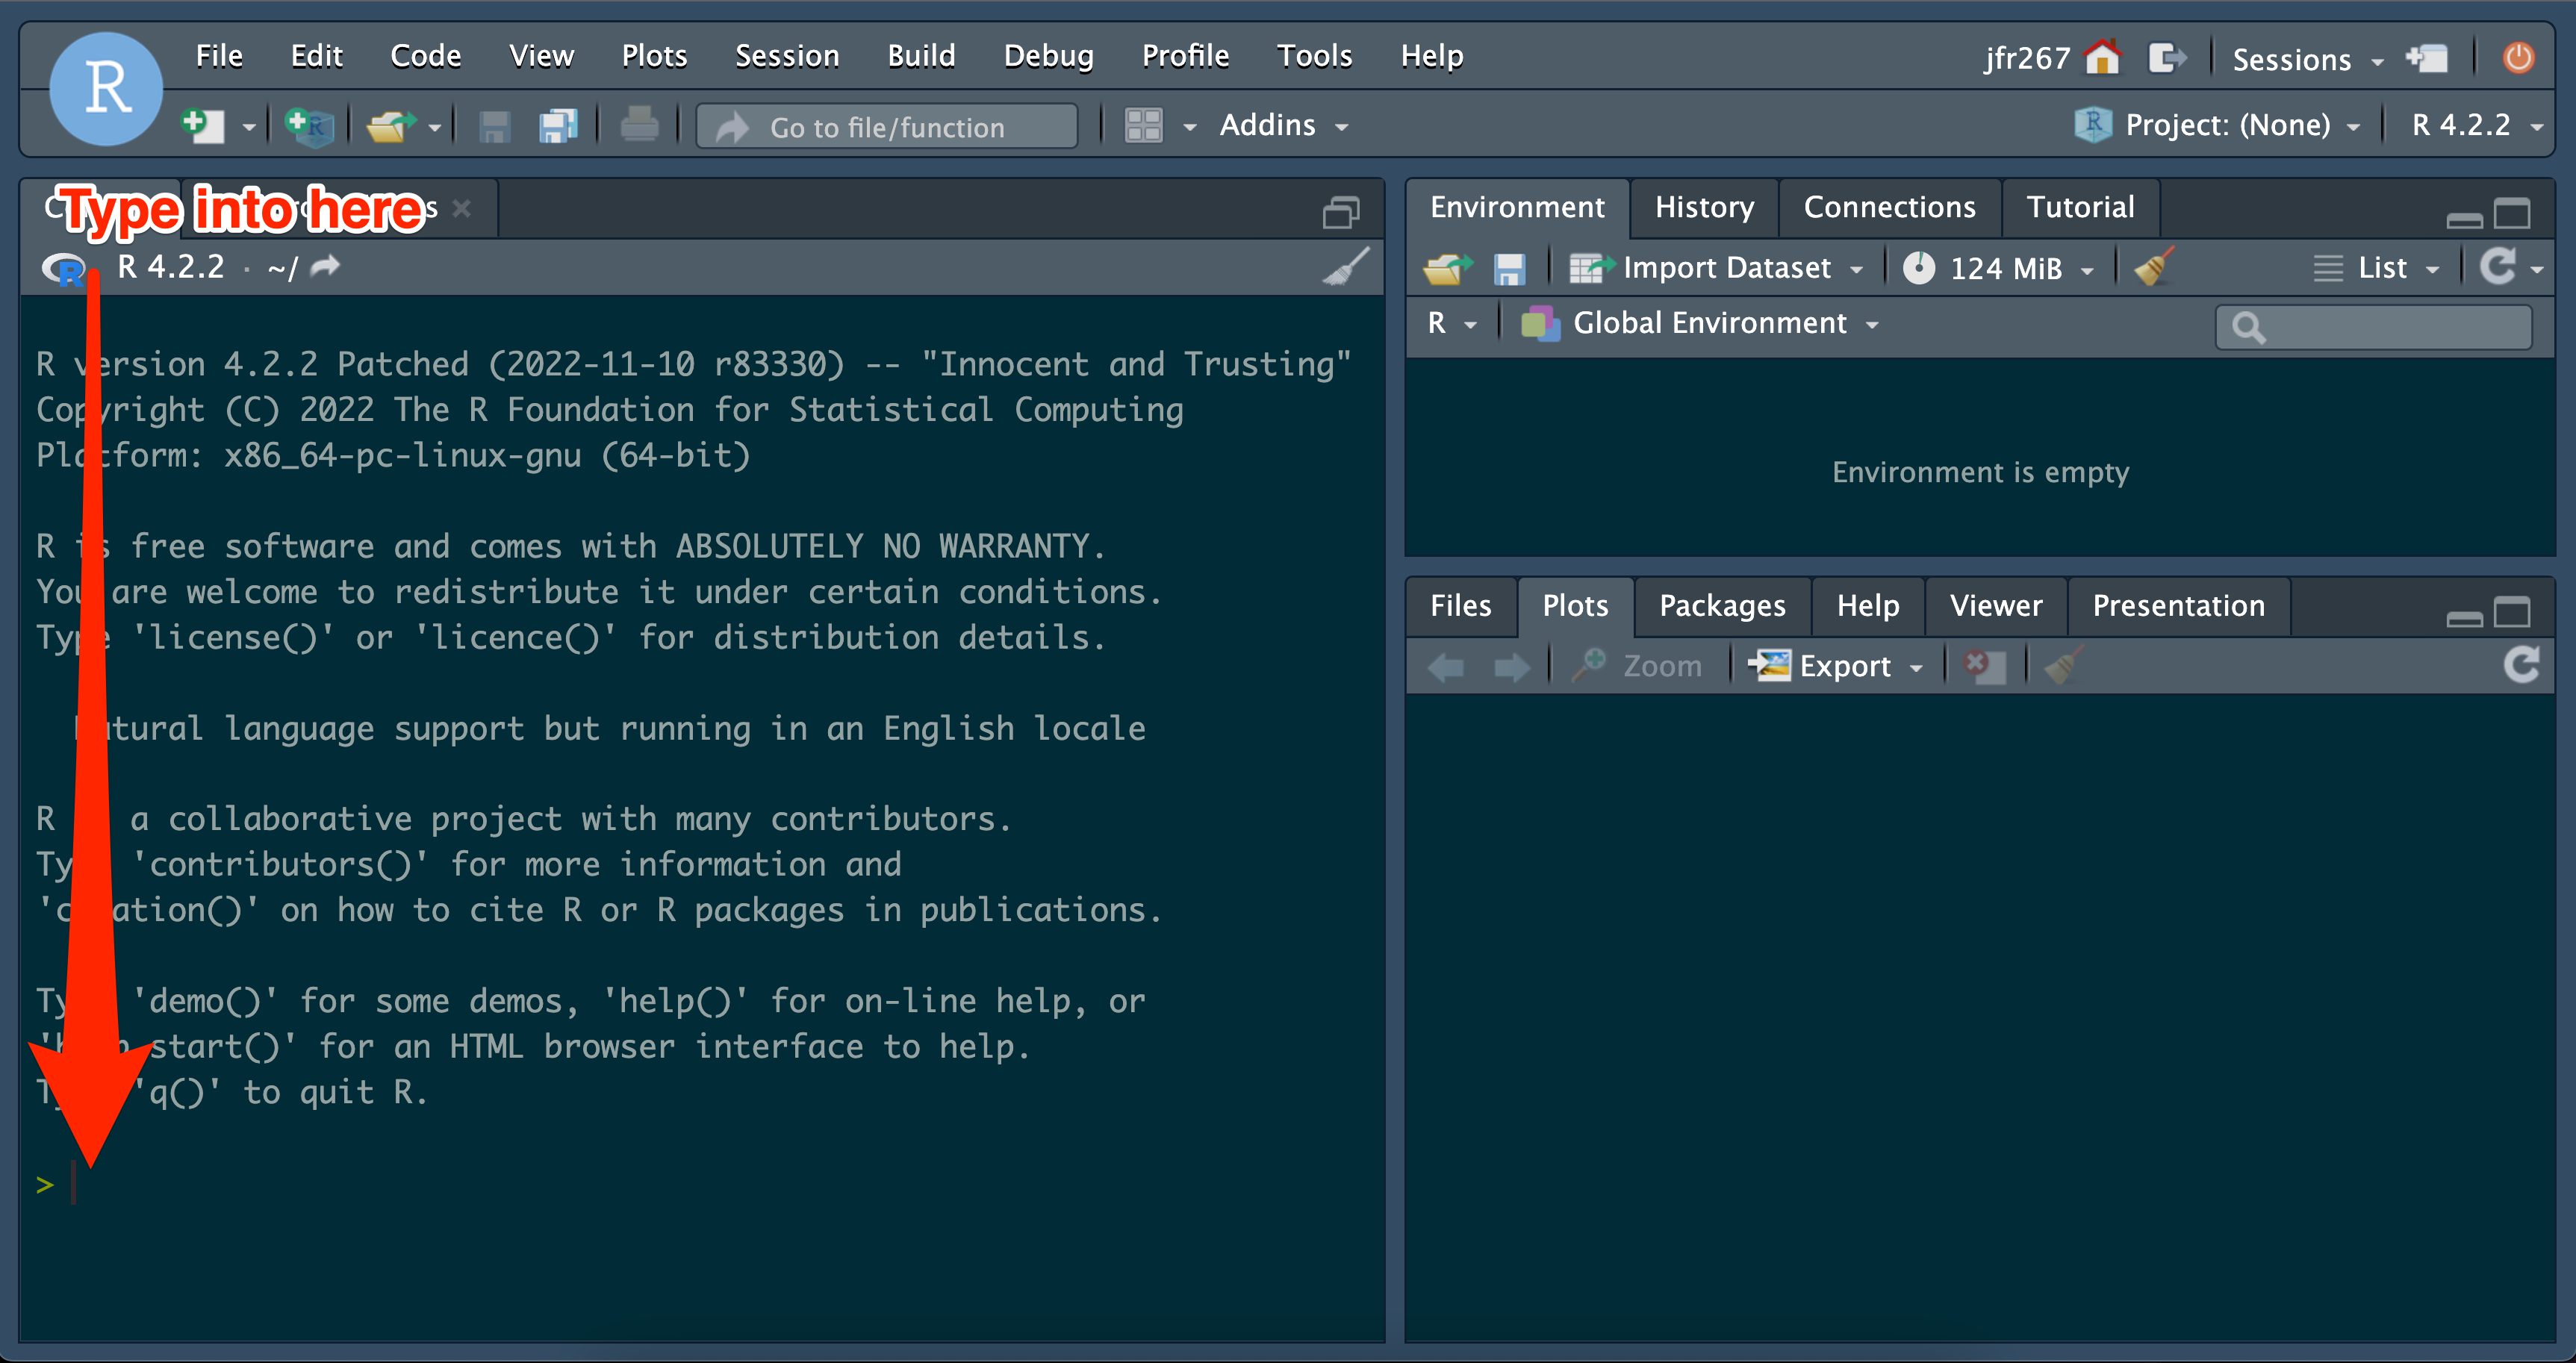
\includegraphics{github_onboarding_assets/rstudio_console.png}

}

\caption{The Console in RStudio is here.}

\end{figure}

Next, we need to tell the local version of Git who you are, specifically
your username (which should match your Github username) and your email
address (which should match the email address you registered for Github
with).

\begin{tcolorbox}[enhanced jigsaw, leftrule=.75mm, colback=white, left=2mm, bottomrule=.15mm, rightrule=.15mm, breakable, arc=.35mm, opacityback=0, colframe=quarto-callout-tip-color-frame, toprule=.15mm]

\textbf{\faIcon{r-project}, \faIcon{git}}\vspace{2mm}

In the code below, \texttt{USERNAME} should be replaced with your Github
username and \texttt{EMAIL} should be replaced with the email you
registered your github account with.

\textbf{Run this in the R Console:}

\begin{Shaded}
\begin{Highlighting}[]
\FunctionTok{system}\NormalTok{(}\StringTok{\textquotesingle{}git config {-}{-}global user.name "USERNAME"\textquotesingle{}}\NormalTok{)}
\FunctionTok{system}\NormalTok{(}\StringTok{\textquotesingle{}git config {-}{-}global user.email "EMAIL"\textquotesingle{}}\NormalTok{)}
\end{Highlighting}
\end{Shaded}

\end{tcolorbox}

\hypertarget{step-3-configure-rstudio-to-communicate-with-github}{%
\subsection{Step 3: Configure RStudio to Communicate with
Github}\label{step-3-configure-rstudio-to-communicate-with-github}}

In order to be able to push commits from RStudio to Github, you'll need
to set up secure communication between wherever you are using RStudio
and Github. I'll walk you through how to do this with SSH credentials.
(See also \href{https://happygitwithr.com/https-pat.html}{Happy Git with
R} for personal access tokens via HTTPS).

\hypertarget{rstudio-configuration}{%
\subsubsection{RStudio Configuration}\label{rstudio-configuration}}

\begin{tcolorbox}[enhanced jigsaw, leftrule=.75mm, colback=white, left=2mm, bottomrule=.15mm, rightrule=.15mm, breakable, arc=.35mm, opacityback=0, colframe=quarto-callout-tip-color-frame, toprule=.15mm]

\textbf{\faIcon{r-project}}\vspace{2mm}

\begin{description}
\item[Go To:]
The Tools menu, then Global Options
\end{description}

\begin{figure}[H]

{\centering 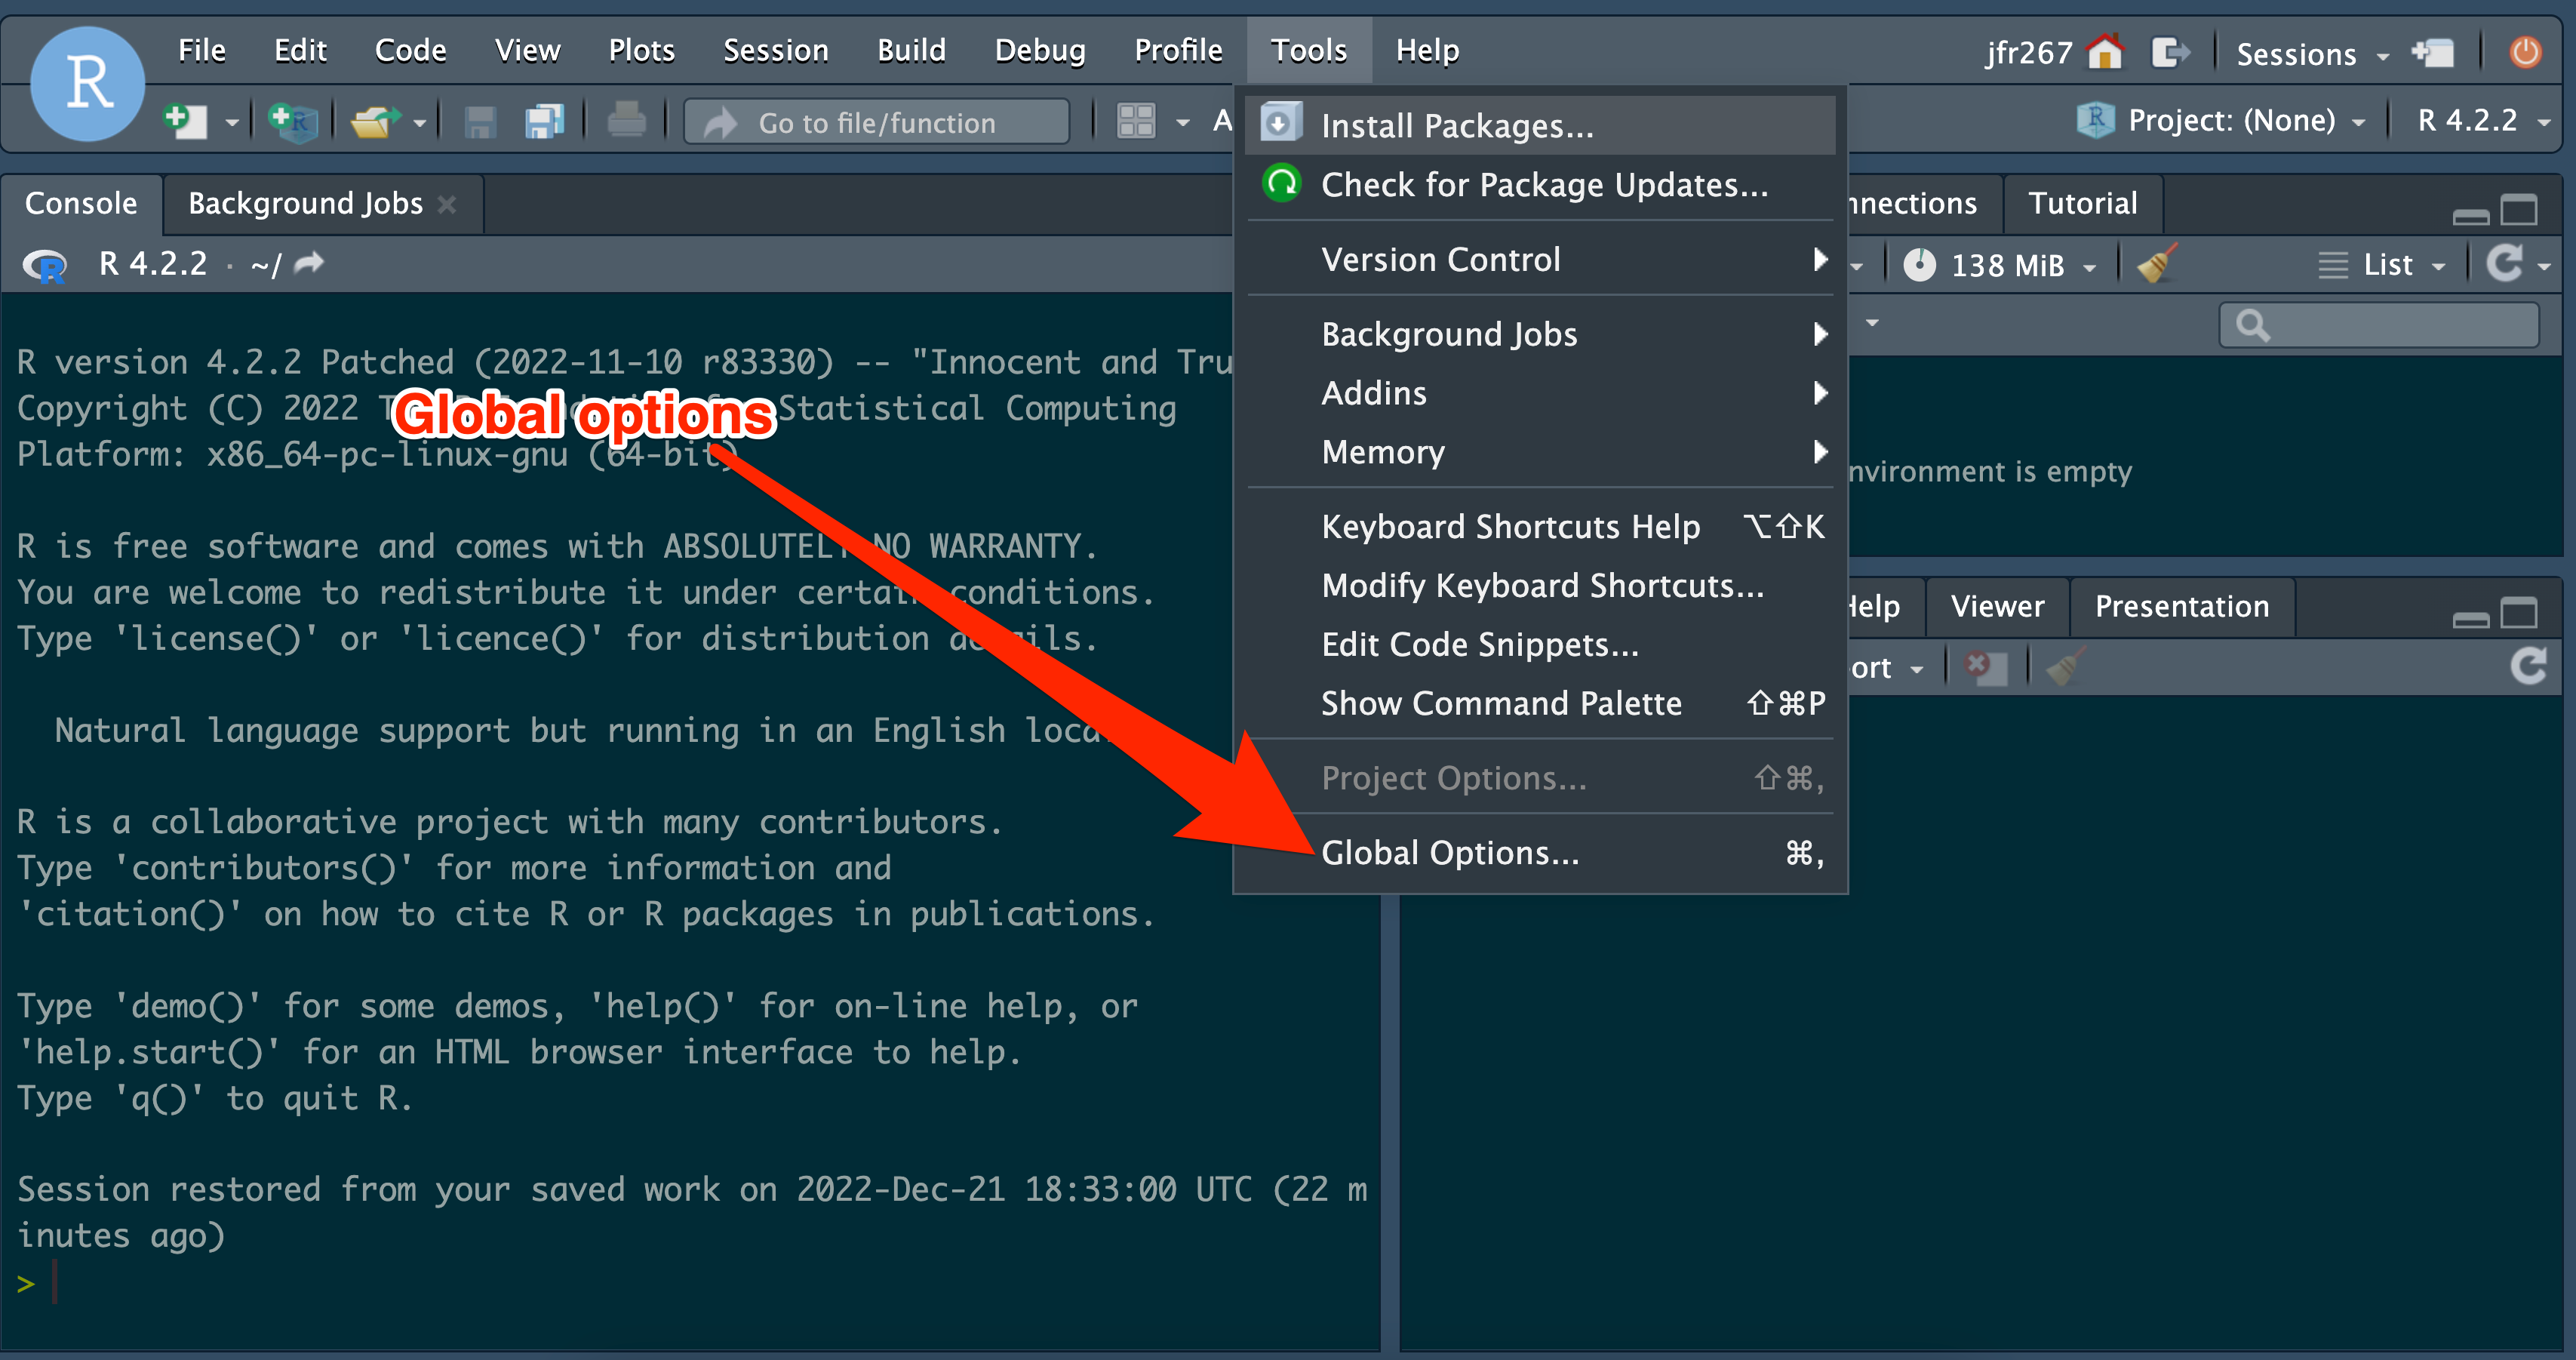
\includegraphics[width=0.76\textwidth,height=\textheight]{github_onboarding_assets/global_options.png}

}

\end{figure}

\begin{description}
\item[Then Go To:]
Git/SVN from the left hand side option selector. Its icon is a cardboard
box
\end{description}

\begin{figure}[H]

{\centering 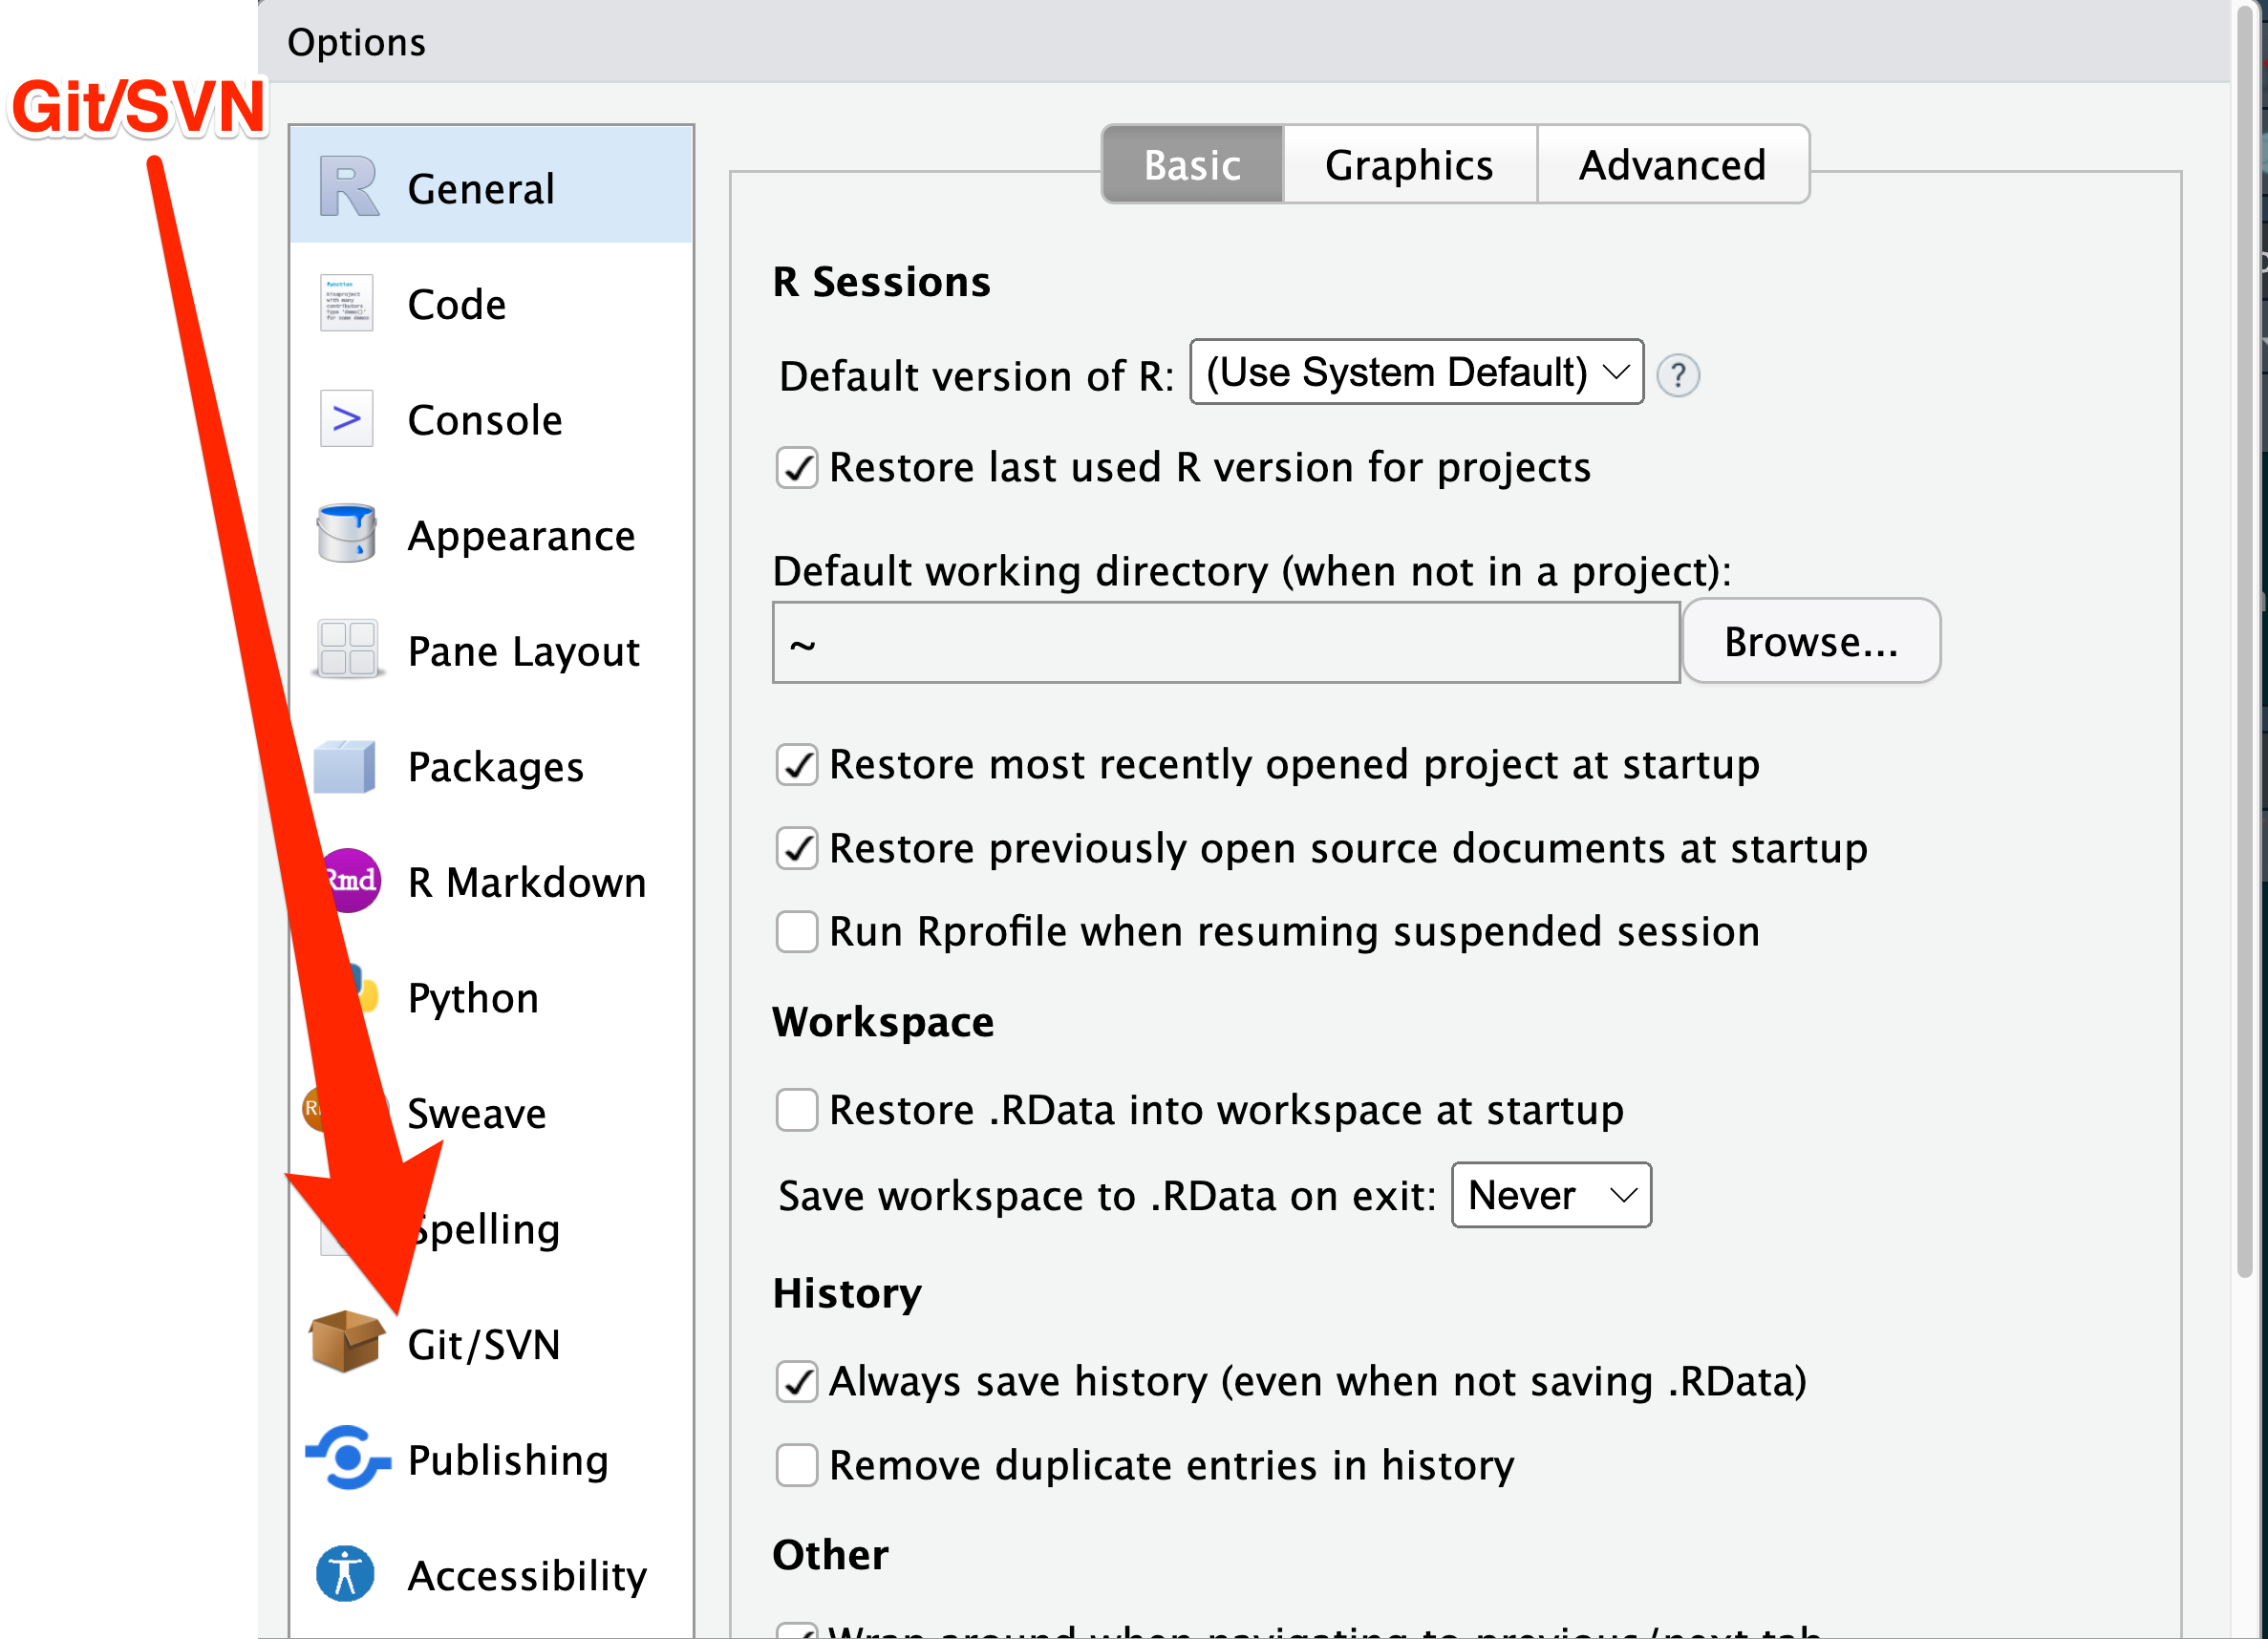
\includegraphics[width=0.75\textwidth,height=\textheight]{github_onboarding_assets/git_svn.png}

}

\end{figure}

\begin{description}
\item[Then Go To]
Create SSH Key
\end{description}

\begin{figure}[H]

{\centering 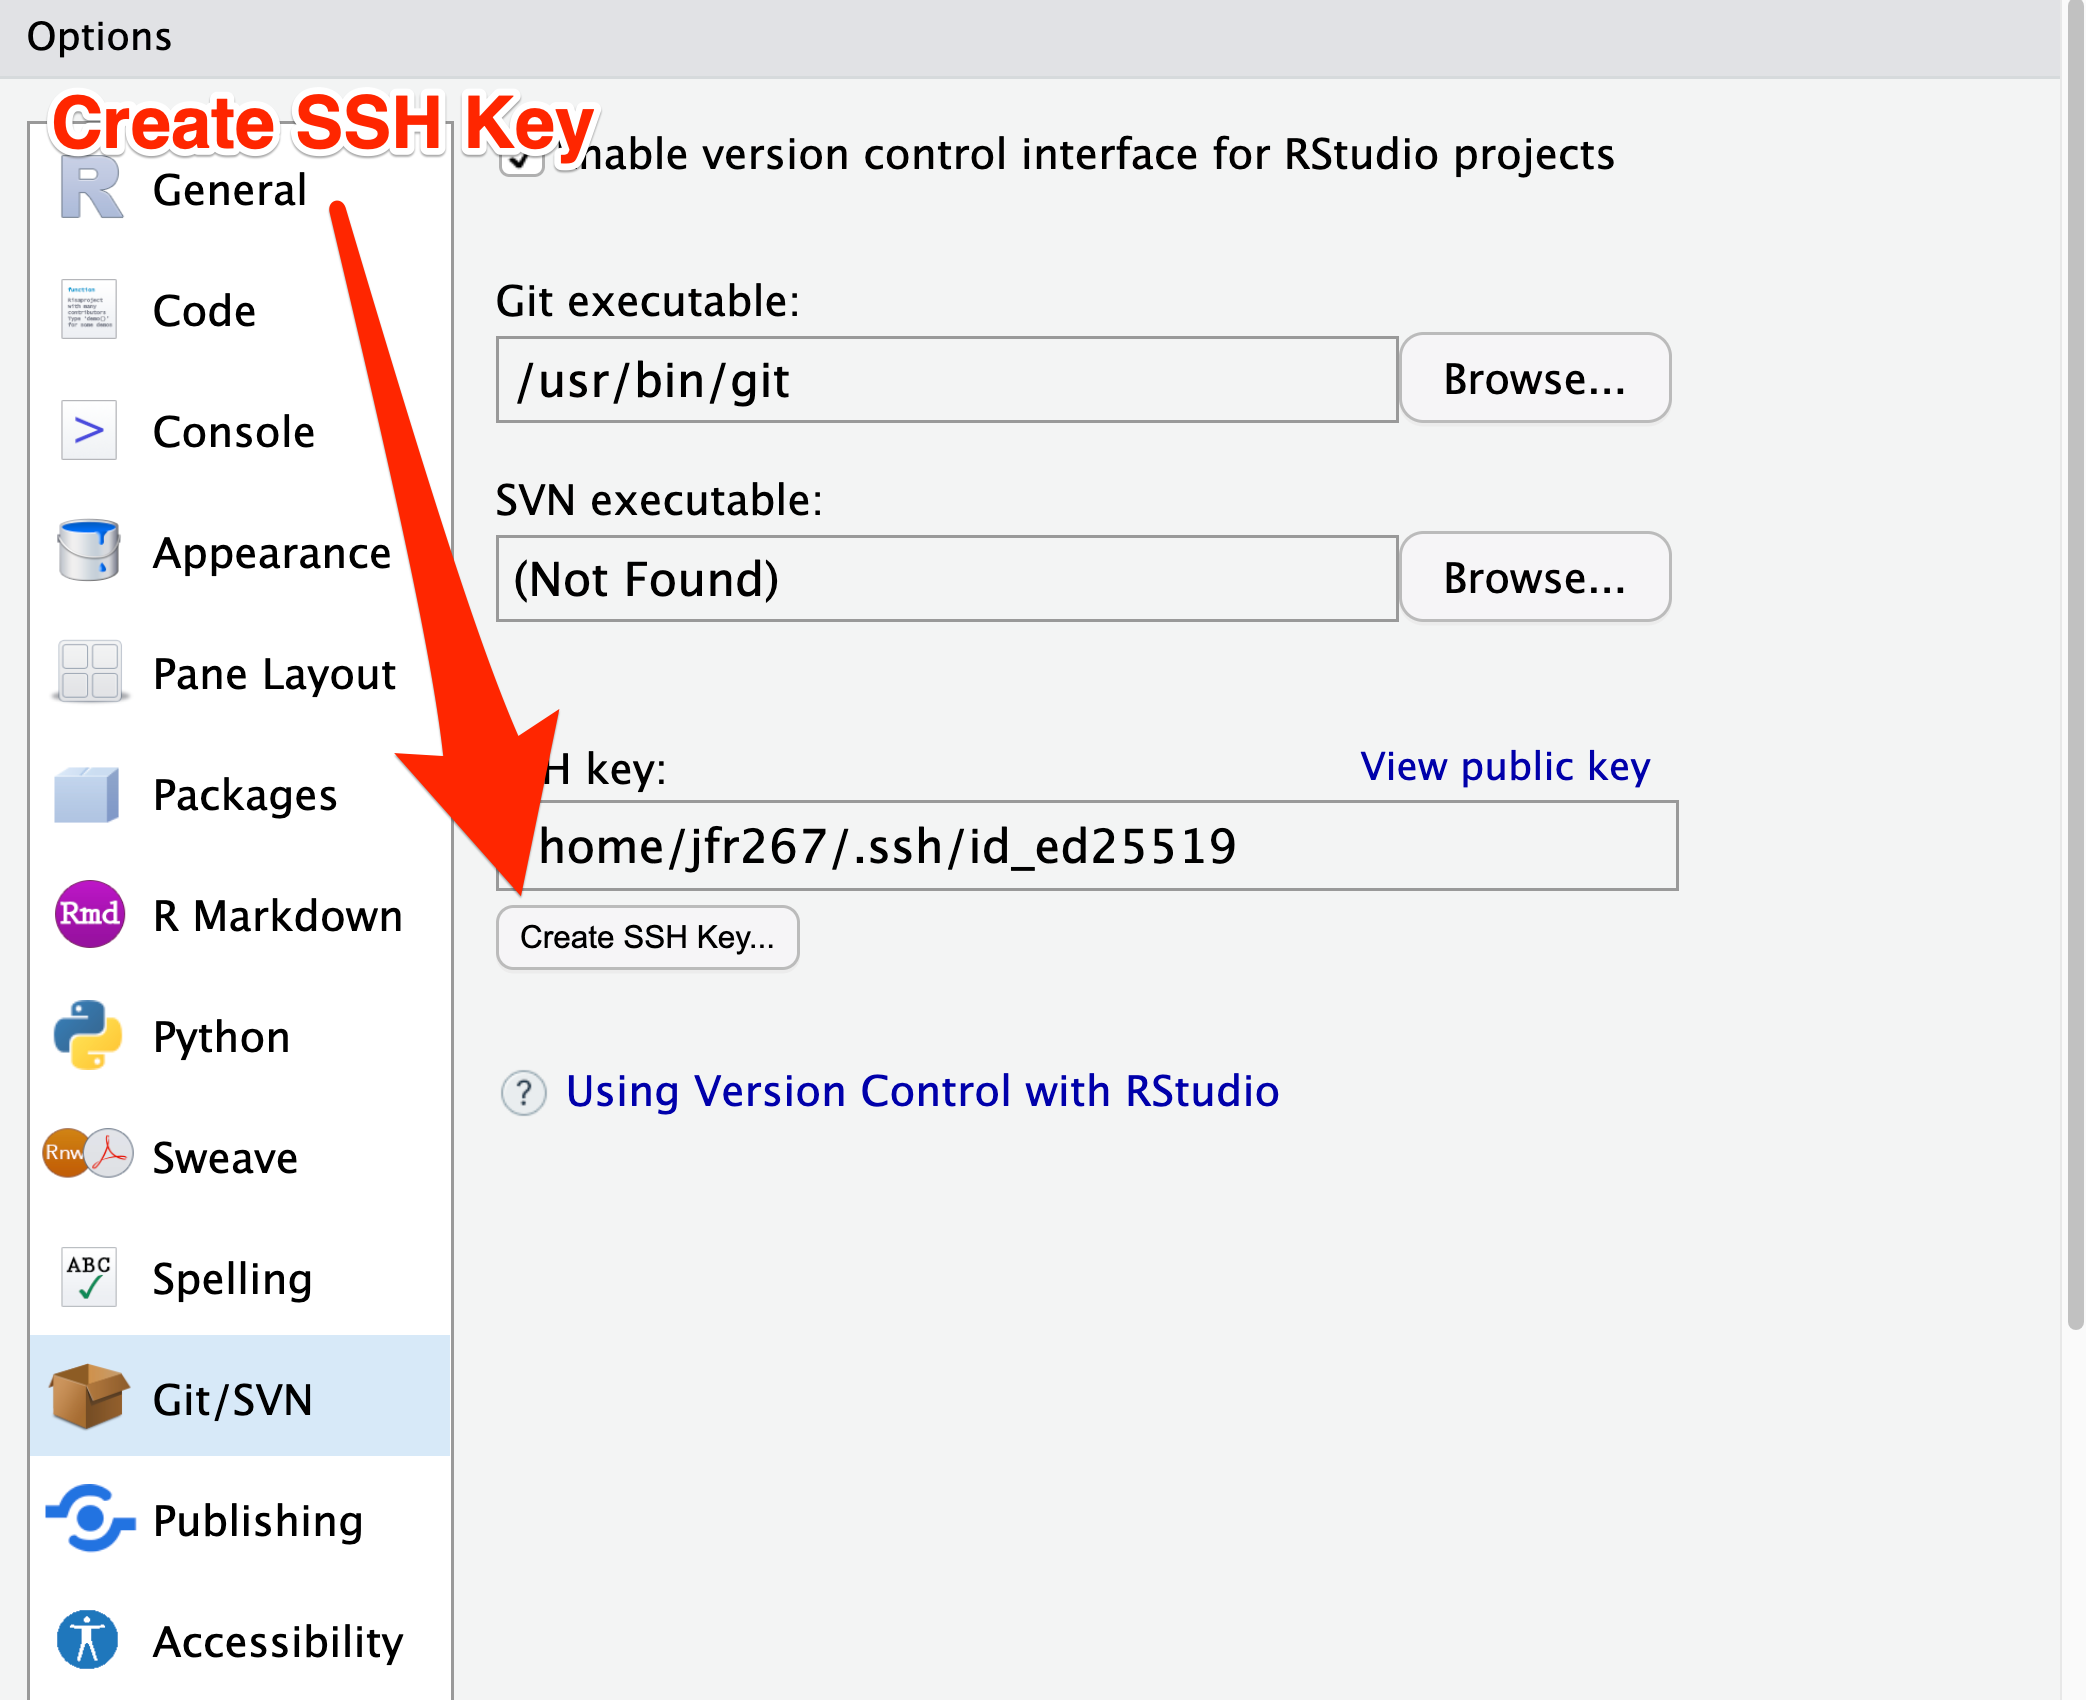
\includegraphics[width=0.75\textwidth,height=\textheight]{github_onboarding_assets/create_ssh_key.png}

}

\end{figure}

\begin{description}
\item[Then]
The default options should be fine to use. The passphrase here is
\emph{\textbf{for the ssh key}.} It should \uline{\textbf{\emph{not}}}
be your Github password, or the password for logging into Posit
Workbench or Posit Cloud. Once you're ready, click Create.
\item[Then]
After creating the SSH key, you should see the option ``View Public
Key''. Click on it, and copy the text that appears.
\end{description}

\end{tcolorbox}

This concludes everything necessary on the RStudio side of things. You
should probably keep the session open so that you can come back to
re-copy your public key.

\hypertarget{github-configuration}{%
\subsubsection{Github Configuration}\label{github-configuration}}

Now, you'll need to go over to github to add the public key to your
profile.

\begin{tcolorbox}[enhanced jigsaw, leftrule=.75mm, colback=white, left=2mm, bottomrule=.15mm, rightrule=.15mm, breakable, arc=.35mm, opacityback=0, colframe=quarto-callout-tip-color-frame, toprule=.15mm]

\textbf{\faIcon{github}}\vspace{2mm}

\begin{description}
\item[Go To]
Your Github Profile Settings
\end{description}

\begin{figure}[H]

{\centering 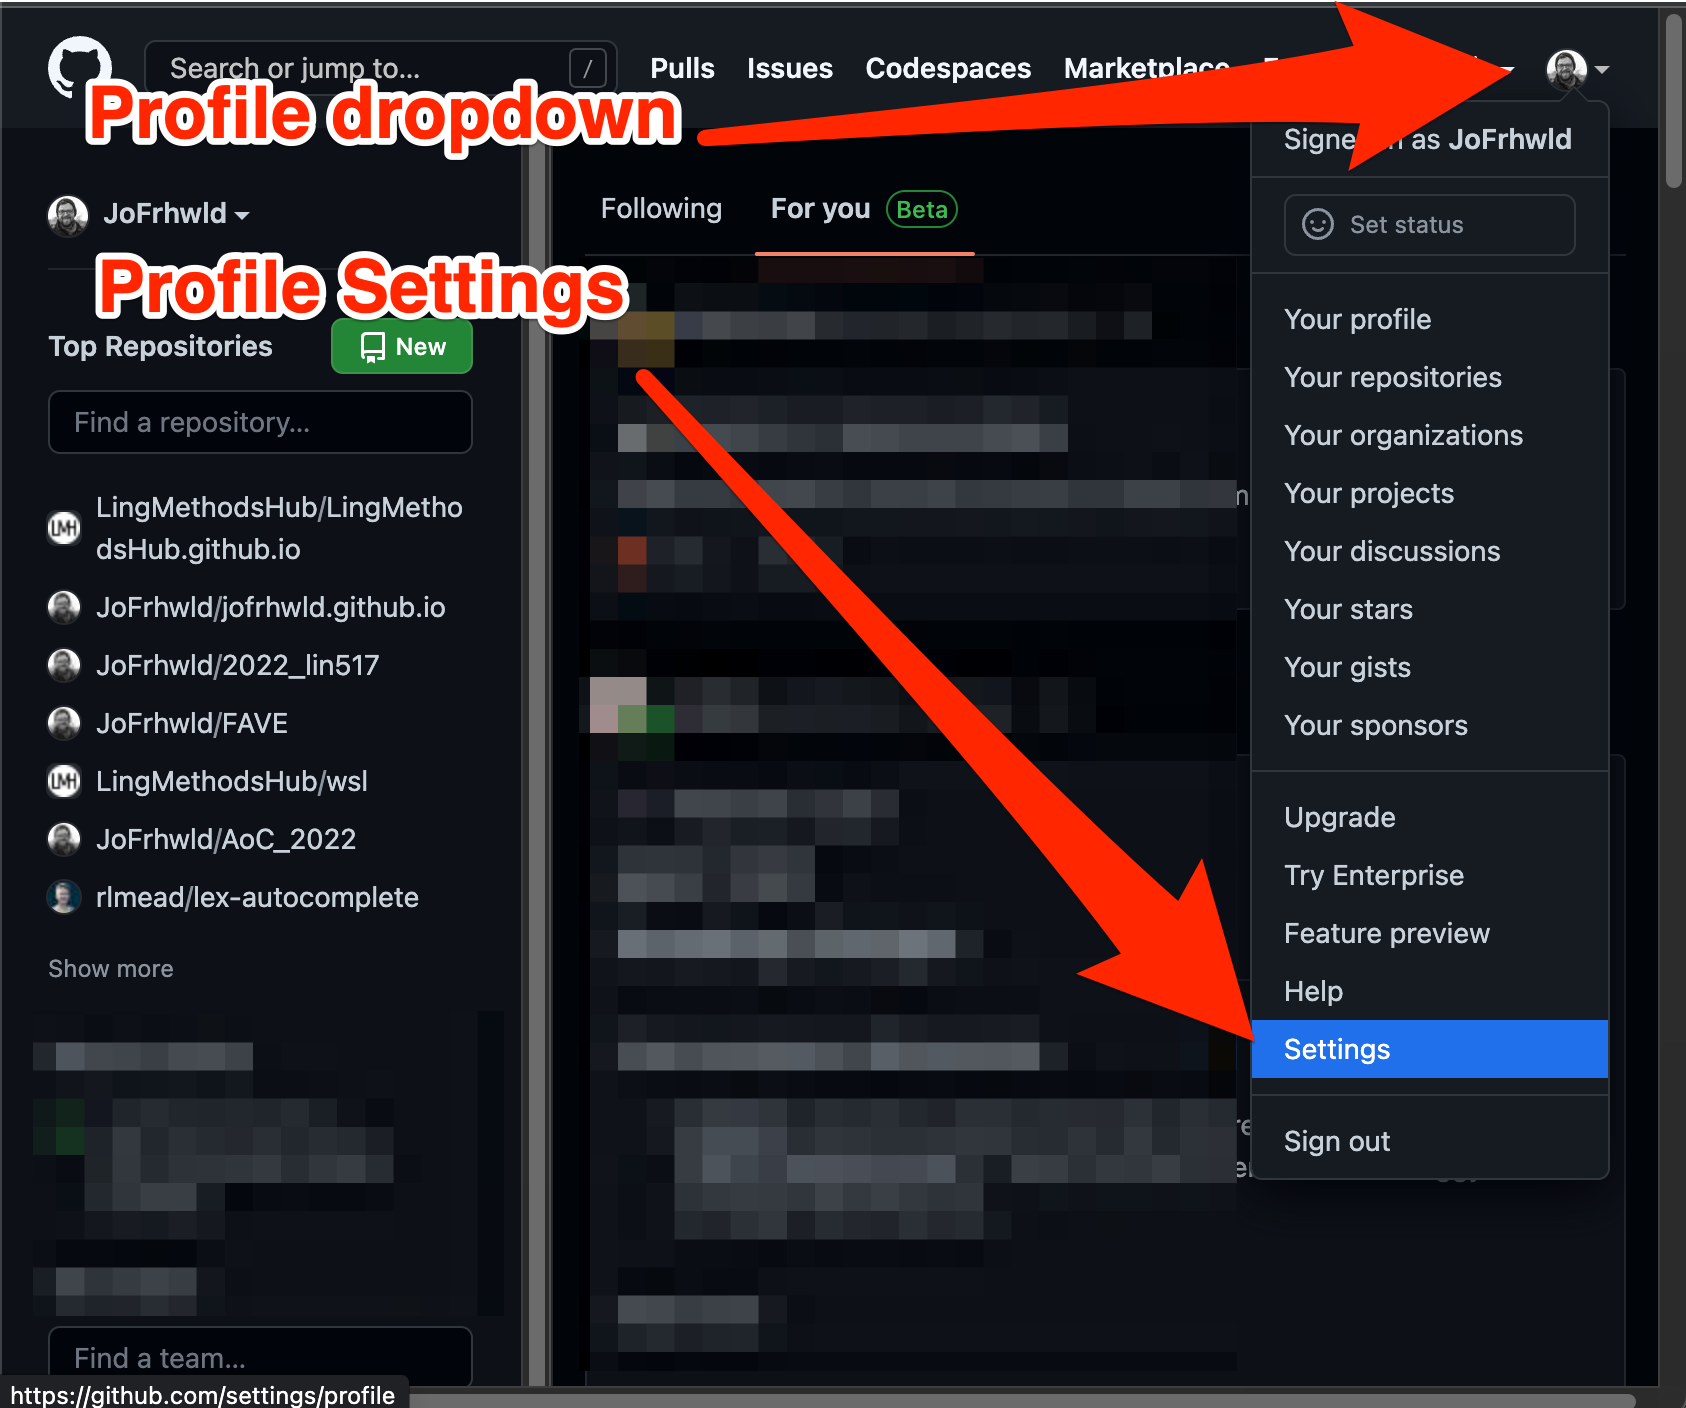
\includegraphics[width=0.75\textwidth,height=\textheight]{github_onboarding_assets/github_settings.png}

}

\end{figure}

\begin{description}
\item[Then Go To]
SSH and GPG keys from the left side menu
\end{description}

\begin{figure}[H]

{\centering 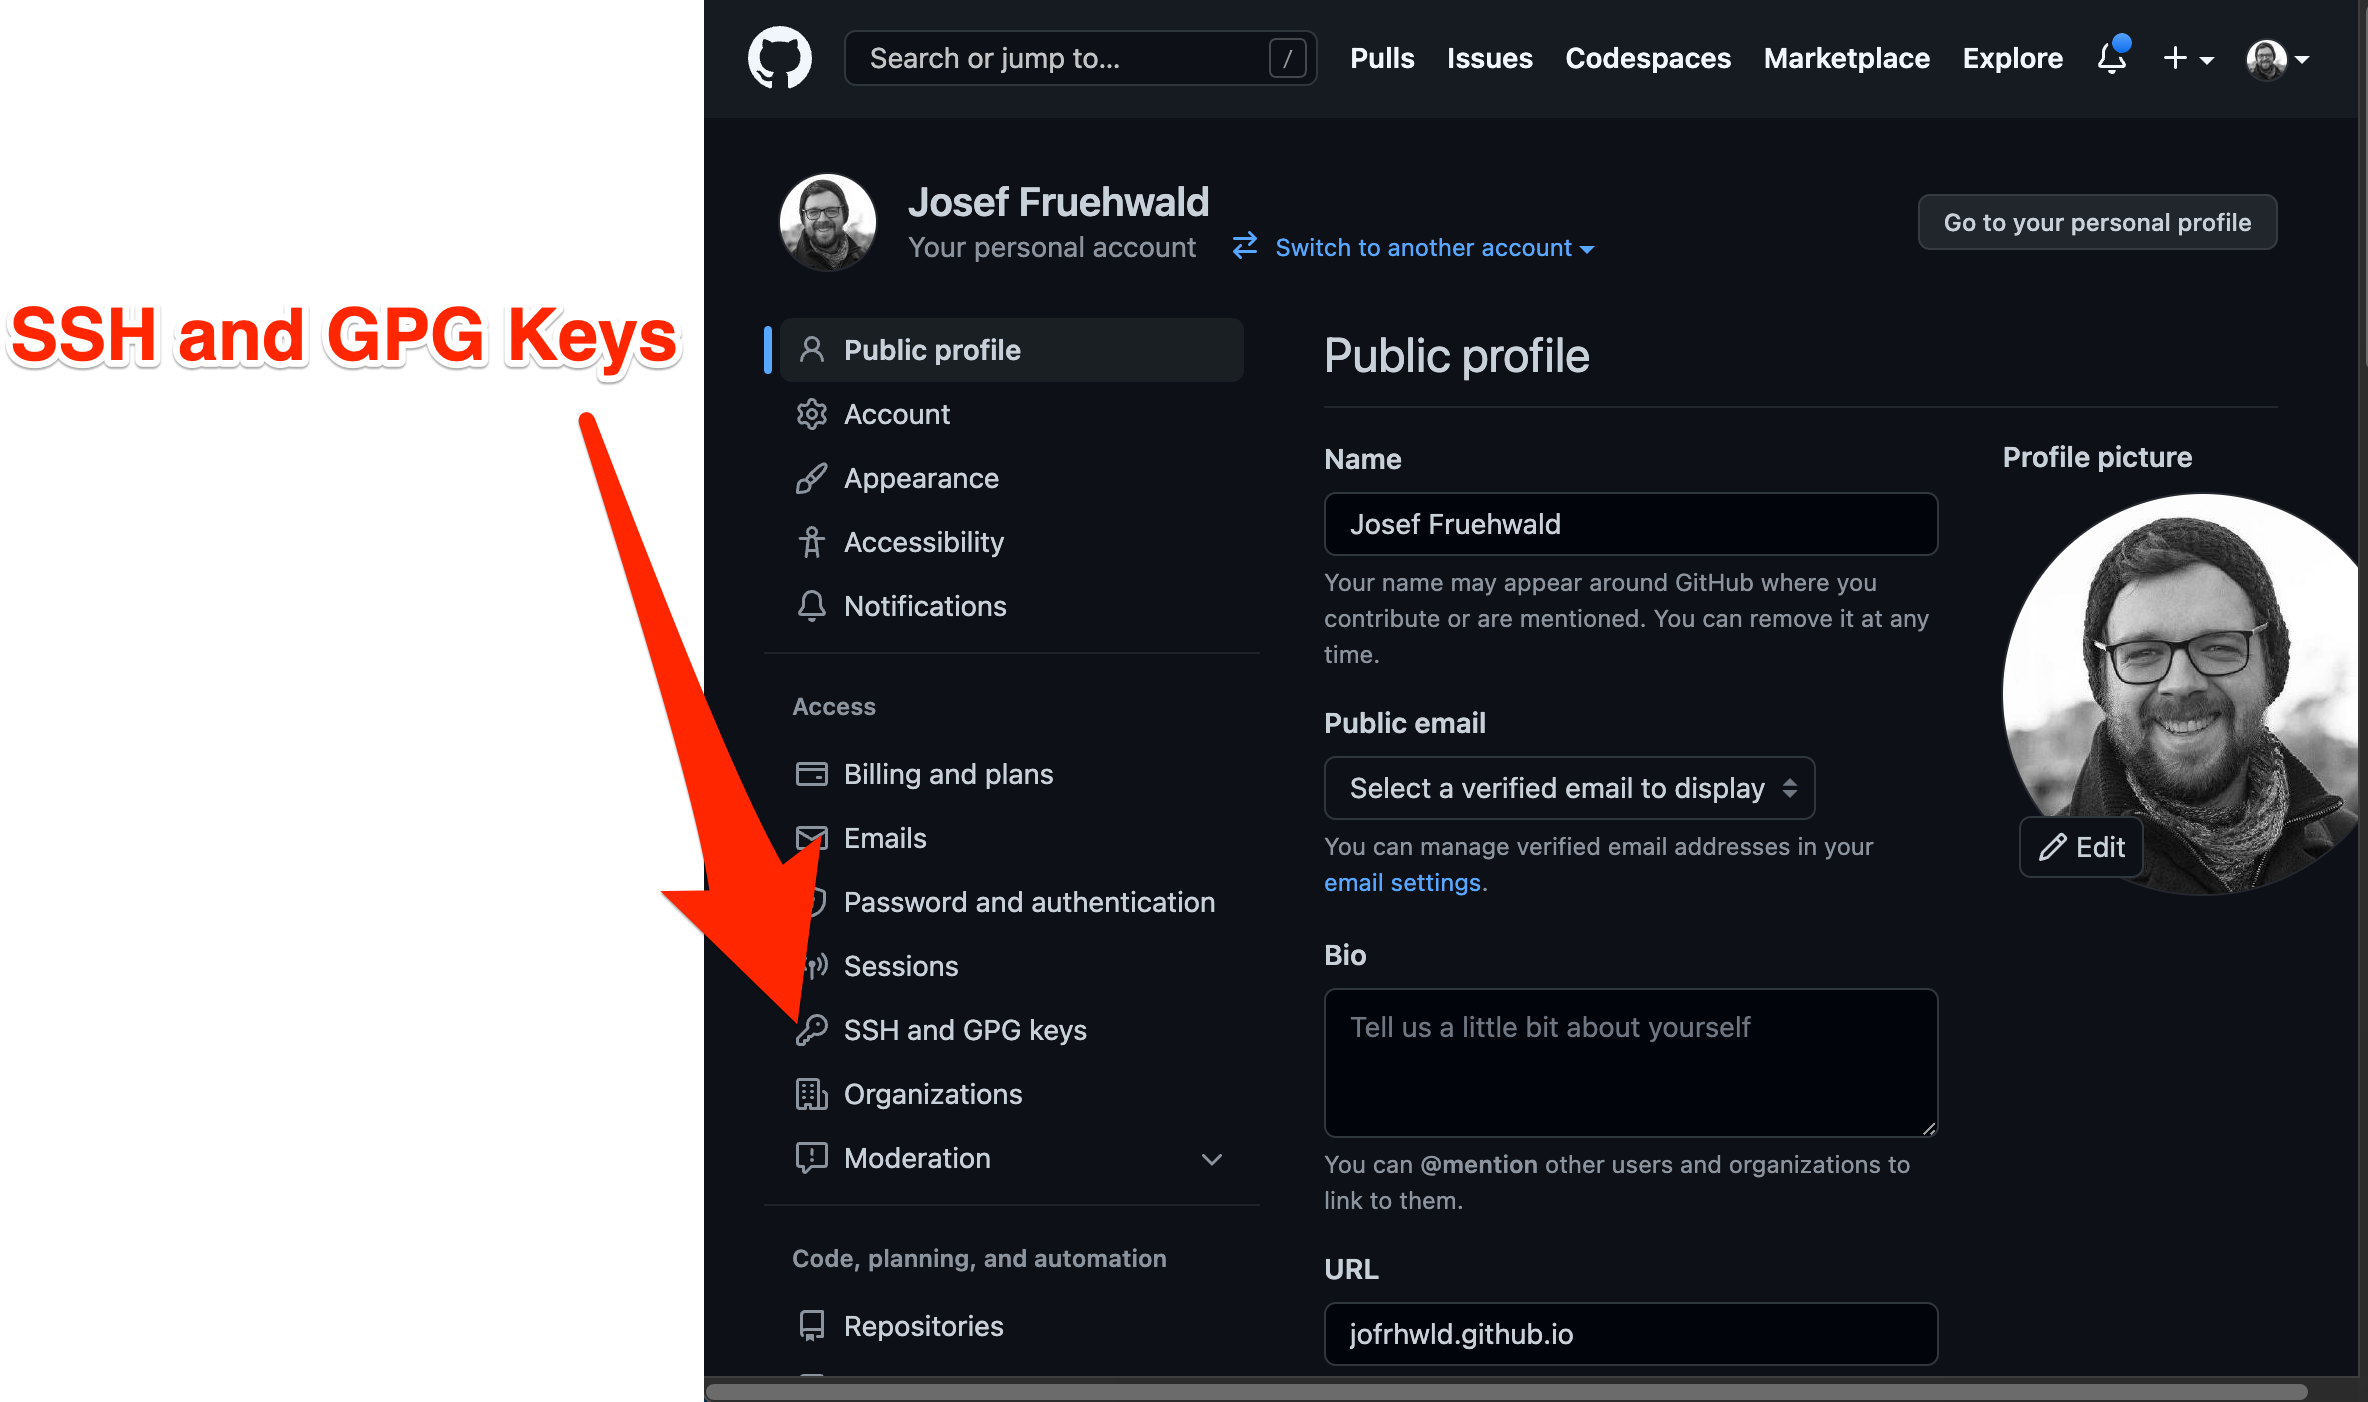
\includegraphics[width=0.75\textwidth,height=\textheight]{github_onboarding_assets/ssh_gpg.png}

}

\end{figure}

\begin{description}
\item[Then]
Click on the New SSH key button
\end{description}

\begin{figure}[H]

{\centering 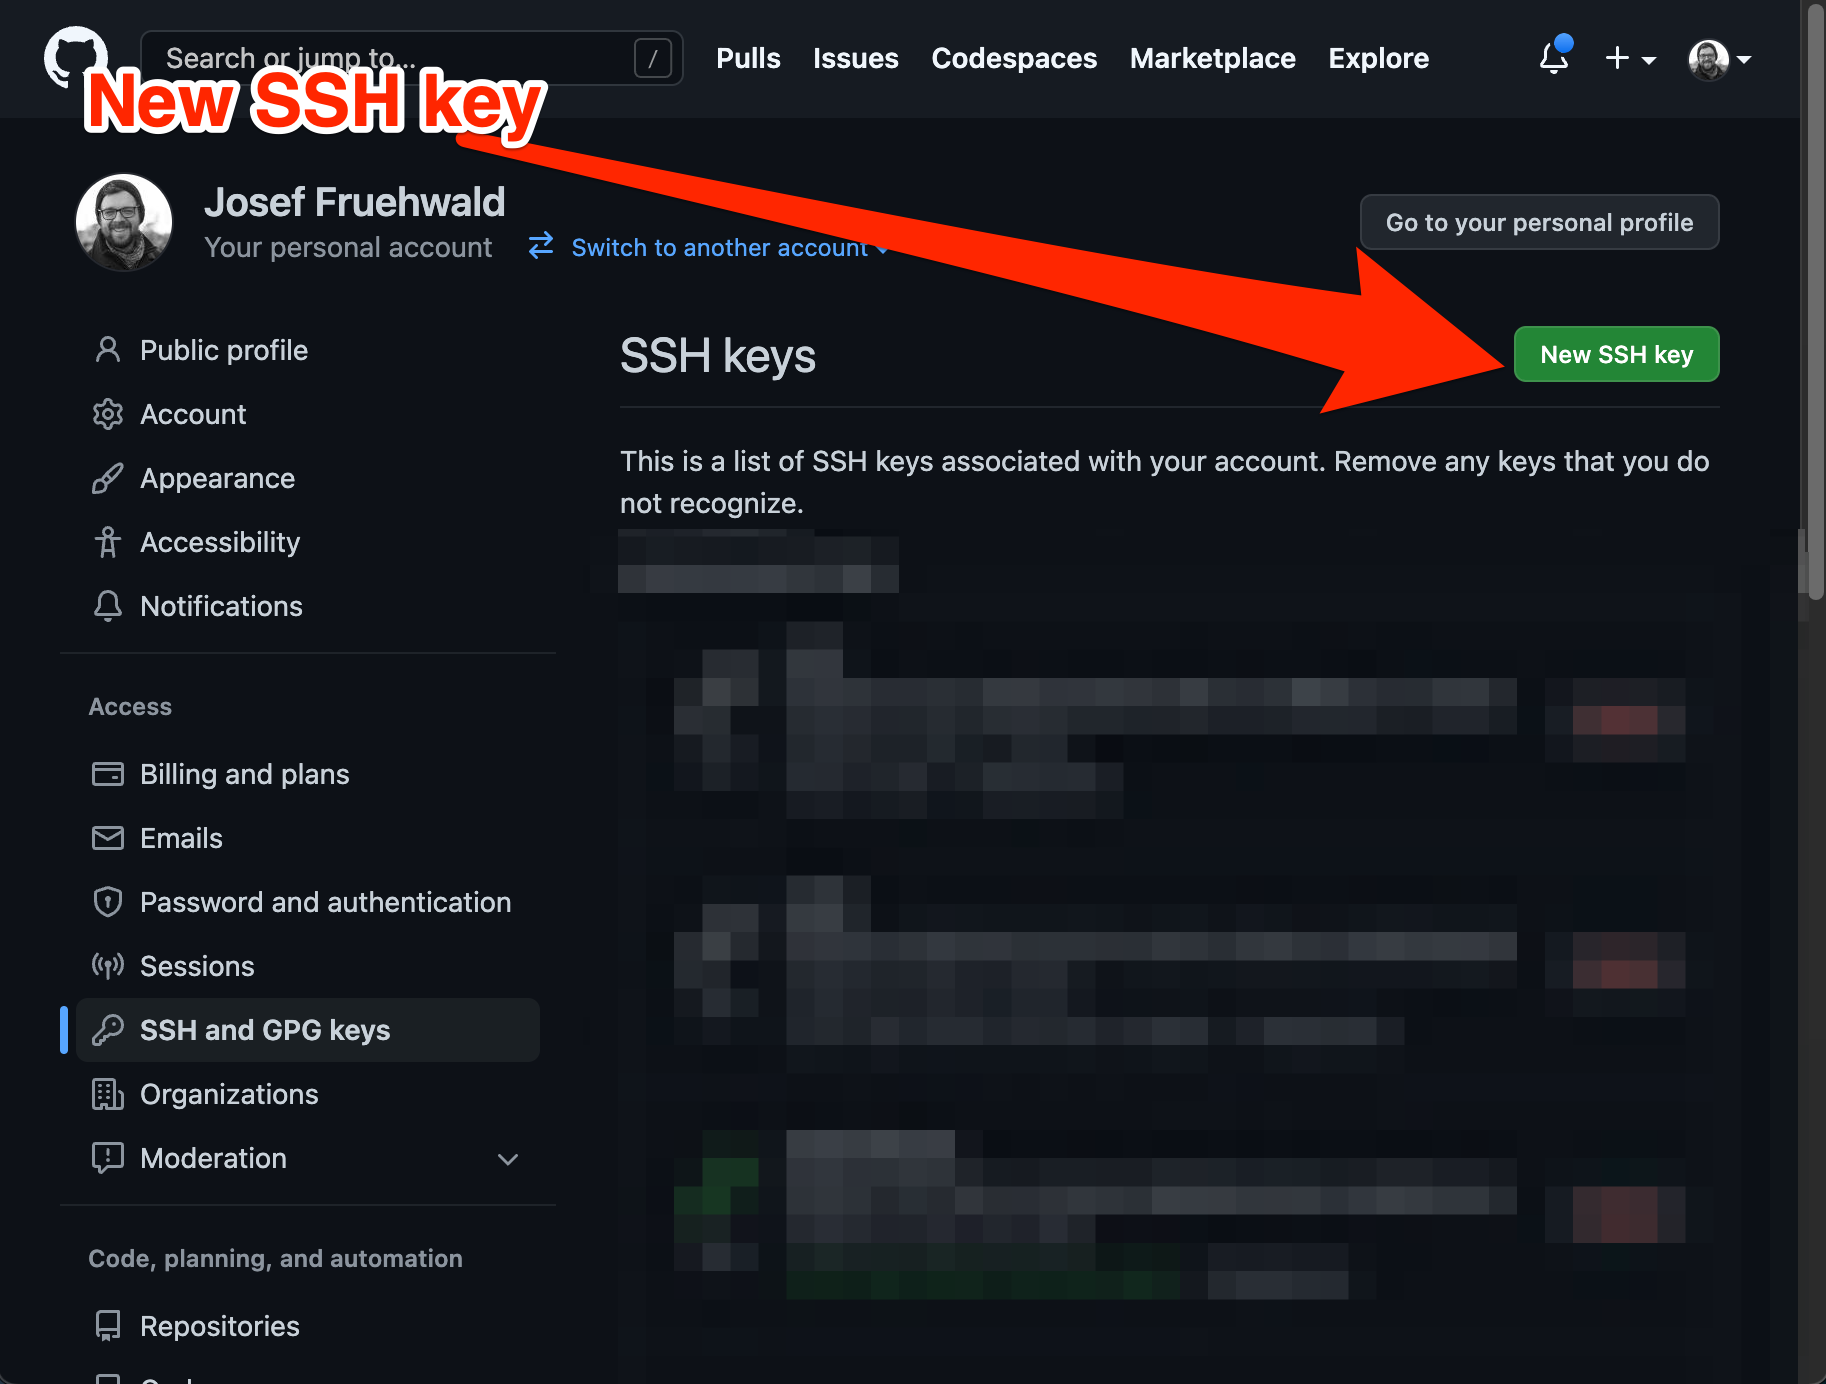
\includegraphics[width=0.75\textwidth,height=\textheight]{github_onboarding_assets/new_ssh_key.png}

}

\end{figure}

\begin{description}
\item[Then]
Give this key an informative name so you can remember which computer
it's coming from.
\item[Then]
Paste the text you copied from RStudio into the Key box and click Add
SSH Key.
\end{description}

\end{tcolorbox}

\hypertarget{configured}{%
\subsection{Configured}\label{configured}}

Now, wherever you are using RStudio from should be able to push commits
to your Github account.



\end{document}
